% Manuscript v6 (final, Energy and Buildings submission), after the author's comments on v5
% (paper/manuscript v5 Liang Zhang comments and edits.docx; responses in paper/RESPONSE_author_comments_v2.md).
% v5: manuscript_v5.tex; v4 and earlier: see paper/.
% Target: Energy and Buildings (Elsevier, elsarticle, numbered citations).
% Compile: pdflatex manuscript_v6_final && bibtex manuscript_v6_final && pdflatex manuscript_v6_final (twice), or Overleaf.
\documentclass[preprint,12pt]{elsarticle}
\usepackage{amsmath,amssymb,graphicx,booktabs,siunitx,hyperref,xcolor}
\usepackage[switch]{lineno}
\linenumbers
\biboptions{numbers,sort&compress}
\graphicspath{{../results/figures/}}
\journal{Energy and Buildings}

\begin{document}
\begin{frontmatter}
\title{Evaluating cooling tower evaporation models for data center water use in building energy simulation}

\author[a,b]{Liang Zhang\corref{cor1}}
\cortext[cor1]{Corresponding author}
\ead{liangzhang1@arizona.edu}
\affiliation[a]{organization={University of Arizona}, city={Tucson}, state={AZ}, country={USA}}
\affiliation[b]{organization={National Laboratory of the Rockies}, city={Golden}, state={CO}, country={USA}}

\begin{abstract}
Cooling towers dominate the direct water use of data centers, yet building energy simulation estimates their
evaporation with simplified relations of unknown error. This study compares eight evaporation models, from
rules of thumb and saturated-exit energy balances to the Poppe model, which resolves the Lewis factor, the evaporated
mass and supersaturated exhaust air. All models are evaluated at the same simulated operating point in every timestep,
with fan-cycling towers resolved into their fan-on and free-convection states, so that differences isolate evaporation physics. The models are implemented as an open-source EnergyPlus plugin, verified against an
independent solution and 126 measured fill tests, and applied in 14 climates to the U.S. Department of Energy large data
center prototype, a data center with a variable-speed tower and the large office prototype. The error
of simplified models follows the state of the exhaust air: saturated-exit models overpredict where hot, dry air leaves
unsaturated and underpredict where cold air leaves supersaturated, and the tower's air-to-water ratio decides which
regime dominates. The EnergyPlus default differs from Poppe by -9 to +38\,\% in annual evaporation; for the
data center prototype, up to 22 percentage points come from averaging fan cycling over the timestep. Empirical rules
deviate by up to 65\,\%, and local makeup-water chemistry changes makeup by -16 to +44\,\%. Data center water estimates
for design, siting and the choice between air-cooled and evaporative heat rejection should use a model that resolves
the exhaust-air state and part-load operation, and should state the cycles of concentration assumed.
\end{abstract}

\begin{highlights}
\item Eight cooling tower evaporation models compared inside EnergyPlus simulations
\item Errors of simple models follow the state of the air leaving the tower
\item Simple models overpredict in hot, dry air and underpredict in cold air
\item Default EnergyPlus method differs from Poppe by up to 38\,\% for a data center
\item Open-source EnergyPlus plugin makes the physics-based models available to all
\end{highlights}

\begin{keyword}
Cooling tower \sep Evaporation \sep Data center \sep Water use \sep Poppe method \sep Building energy simulation \sep
EnergyPlus
\end{keyword}
\end{frontmatter}

\section*{Nomenclature}
\begin{tabular}{ll}
$B$, $D_r$ & blowdown, drift [kg/s] \\
$c_{pa}, c_{pv}, c_{pw}$ & specific heat of dry air, vapour, liquid water [J/(kg\,K)] \\
$\mathcal{D}$ & denominator of the Poppe equations, Eq.~(2) [J/kg] \\
$E$ & evaporation rate [kg/s] (annual totals in m$^3$) \\
$f$ & fan-on fraction of a timestep (fan-cycling tower) [--] \\
$i_{ma}$, $i_{masw}$ & enthalpy of moist air; of saturated air at $T_w$ [J/kg dry air] \\
$i_{fg}$, $i_v$ & latent heat; vapour enthalpy at $T_w$ [J/kg] \\
$K$ & mass transfer coefficient times area [kg/s] \\
$L/G$ & water-to-dry-air mass flow ratio [--] \\
$Le_f$ & Lewis factor [--] \\
$Me_P$ & Poppe Merkel number [--] \\
$\dot m_a$, $\dot m_w$ & dry-air and water mass flow [kg/s] \\
$N_c$, $N_{c,\mathrm{eff}}$ & cycles of concentration; effective annual value $E/(B+D_r)+1$ [--] \\
$NTU$ & number of transfer units (Braun model) [--] \\
$\dot Q$ & heat rejected, $\dot m_{w}c_{pw}(T_{w,i}-T_{w,o})$ [W] \\
$T_{db}$, $T_{wb}$, $T_w$ & dry-bulb, wet-bulb, water temperature [\textdegree C] \\
$\Delta T$ & cooling range, $T_{w,i}-T_{w,o}$ [K] \\
$\omega$, $\omega_{sw}$ & humidity ratio; saturated at $T_w$ [kg/kg dry air] \\
$\omega_{se}$ & humidity ratio of saturated air at the effective saturation enthalpy (Braun model) [kg/kg dry air] \\
Subscripts $i$, $o$ & inlet, outlet \\
L/kWh$_{th}$ & litres of evaporation per kWh of heat rejected \\
\end{tabular}

%======================================================================
\section{Introduction}\label{sec:intro}
%======================================================================
Evaporative cooling towers reject the condenser heat of most large chilled-water plants. In commercial and
institutional buildings they are often the largest single water use, 20--50\,\% of a facility's total
\citep{epa2012watersense}, and in data centers, which convert almost all of their electricity into heat and reject it
throughout the year, they dominate direct water use \citep{mytton2021data,shehabi2016united}. National assessments
estimate the water use of data centers and its growth \citep{shehabi2024united}, locate it in water-stressed basins
\citep{siddik2021environmental}, and show that their water usage effectiveness (WUE), the site water use per unit of
information technology (IT) energy \citep{greengrid2011wue}, varies widely with climate and cooling technology
\citep{lei2022climate}; the water footprint of computing, including artificial intelligence workloads, has become a
public concern \citep{ristic2015water,li2025making}. Design-stage studies compare the energy and water use of cooling
options \citep{karimi2022water,karimi2025energy}, and water use is increasingly part of building siting, permitting and
reporting. Such estimates need hourly evaporation that is consistent with the simulated plant.

Where water is scarce, these estimates become a design question. In Arizona, the Colorado River entered its first declared shortage in 2022, which cut Arizona's
allocation by about 18\,\%, and a deeper shortage level followed in 2023 \citep{reclamation2021reclamation,
reclamation2022interior}. The state's 100-year groundwater model for the Phoenix Active Management Area projects 4.86
million acre-feet of unmet demand, so that new developments in parts of the region can no longer demonstrate an assured
groundwater supply \citep{azgovernor2023governor,kylcenter2023new}. Cooling towers and chillers have median service
lives of about 20 years \citep{ashrae2015owning}, and the facilities they serve are planned for longer. A heat
rejection system chosen on the water supply and prices of today may therefore operate for decades under tighter
allocations, and a design based on short-term water availability can turn out to be wrong. Air-cooled heat rejection
consumes almost no water on site but uses more energy, especially in hot weather, whereas evaporative towers save energy
at the cost of water \citep{vangeet2024best,karimi2022water,karimi2025energy}; in a hot, arid climate, an air-cooled data
center had a 13\,\% higher power usage effectiveness but a 66\,\% lower source WUE than a water-cooled one
\citep{karimi2022water}. Choosing between air-cooled, hybrid and water-cooled systems, and sizing them for the life of
the facility, requires water consumption estimates that are accurate over the whole range of climates and operating
conditions the plant will see.

Building energy simulation resolves the hourly heat rejected by the plant and is therefore the natural tool for these
estimates. The evaporation that accompanies this heat, however, is computed with simplified relations. EnergyPlus
\citep{crawley2001energyplus}, a widely used open engine, offers a constant loss factor per kelvin of cooling range, or
an energy balance that assumes the exhaust air leaves saturated \citep{doe2022engref}; blowdown follows from a fixed
concentration ratio. \citet{powers2016new} noted that evaporation models in whole-building simulation are either too
simple or too slow for water estimates. In the cooling-tower literature the physics behind these simplifications is well
understood. Merkel's method \citep{merkel1925verdunstungskuhlung} sets the Lewis factor to one, neglects the mass of
water evaporated in the energy balance and assumes saturated exhaust air; the Poppe method \citep{poppe1991berechnung}
retains all three effects and can represent supersaturated (fogging) exhaust \citep{klimanek2009solution}.
\citet{kloppers2005critical,kloppers2005cooling} compared the Merkel, effectiveness--number of transfer units (e-NTU)
\citep{jaber1989design} and Poppe methods \citep{kroger2004air}: they agree closely in heat rejection but differ in
water evaporated, by an amount that depends on the ambient conditions. \citet{kloppers2005lewis} and
\citet{khan2001improved} examined the Lewis factor, \citet{navarro2022critical} recommended Poppe for a new tower design,
\citet{qureshi2006prediction} studied evaporation-loss prediction, and \citet{lucas2009experimental} measured tower
performance with different drift eliminators.

What has not been quantified is how large these model differences are for the annual water use of real buildings,
whose towers run at part load, in varying weather and under the control of a chiller plant. Two features of building
operation make this question different from the full-load comparisons in the literature. First, when a tower operates
depends on the building: a comfort-cooling plant runs mostly in summer, whereas a data center rejects heat in every hour
of the year, including freezing and humid hours in which the exhaust air is supersaturated. Second, how a tower meets
part load depends on its fan control: a variable-speed fan reduces the air flow, whereas a single-speed fan cycles
between full air flow and free convection. Both change the air-to-water ratio and the state of the exhaust air, which,
as shown below, decide whether simplified models over- or underpredict.

This paper therefore treats evaporation physics as the subject and the building simulation as the test platform. It
asks: (i) where in the space of ambient conditions and air-to-water ratios do simplified evaporation models depart from
the Poppe model, and why; (ii) how do the tower's part-load control and the building's load pattern change the annual
result; and (iii) how does the evaporation-model effect compare with the effect of makeup-water chemistry on total
water use? No measured tower evaporation or makeup data are used, so the case-study comparisons are model-to-model:
Poppe serves as the most complete model, not as ground truth, and is checked against measured fill tests where these
allow. The data center is the primary case because water use matters most there and its towers operate in all seasons;
an office building shows how far the conclusions carry to comfort cooling. The contributions are:
\begin{enumerate}
\item a physical explanation, with a climate-general map, of where and why simplified models depart from Poppe
(Sections~\ref{sec:physics} and \ref{sec:map});
\item a method that evaluates all models on the same simulated operating point, including the two states of a
fan-cycling tower, so that differences isolate evaporation physics (Section~\ref{sec:evaluation});
\item verification against an independent solution and 126 measured fill tests (Section~\ref{sec:verification});
\item annual results for prototype data center and office buildings and a variable-speed tower in 14 climates
(Sections~\ref{sec:annual}--\ref{sec:sensitivity});
\item the effect of each site's own makeup water on cycles of concentration and total water use (Section~\ref{sec:wue});
\item an open-source EnergyPlus plugin that makes all models available to other users (Section~\ref{sec:tool} and
Appendix~\ref{app:code}), with a tutorial, at \url{https://github.com/TensorBuildLab/EnergyPlus-HeatRejection-Water};
\item recommendations on which model to use for data center water estimates (Section~\ref{sec:dcrec}).
\end{enumerate}
All models, building models, data and scripts referred to below as supplementary files are in this repository.

%======================================================================
\section{Evaporation physics and models}\label{sec:physics}
%======================================================================
\subsection{Heat and mass transfer in a wet cooling tower}\label{sec:poppe}
In the fill of a counterflow tower, warm water flows down against rising air. Heat leaves the water by evaporation
(latent heat) and by convection to the air (sensible heat), and the water mass lost by evaporation is the quantity of
interest. Three properties of this process determine how much water evaporates for a given heat rejected. (i) The
sensible share of the heat transfer: in cold air a large part of the heat leaves as sensible heat, so less water
evaporates per unit heat; in hot, dry air the air can be cooled by the water, so its sensible heat is added to the
evaporation and more water evaporates than the heat rejected alone would require. (ii) The Lewis factor $Le_f$, the
ratio of the heat and mass transfer coefficients, which sets that sensible share at a given driving force. (iii) The
state of the exhaust air: it may leave unsaturated (typical of hot, dry air or a high air flow), saturated, or
supersaturated, carrying liquid mist (typical of cold, humid air or a low air flow). A model that fixes the exhaust
state, for example at saturation, cannot represent the first and last cases and will over- or underpredict accordingly.

The Poppe model \citep{poppe1991berechnung,kloppers2005critical} keeps all three effects. With the water temperature as
independent variable,
\begin{equation}
\frac{d\omega}{dT_w} = \frac{c_{pw}\,(\dot m_w/\dot m_a)(\omega_{sw}-\omega)}{\mathcal{D}},\quad
\frac{di_{ma}}{dT_w} = \frac{\dot m_w c_{pw}}{\dot m_a}\left[1+\frac{c_{pw}T_w(\omega_{sw}-\omega)}{\mathcal{D}}\right],\quad
\frac{dMe_P}{dT_w} = \frac{c_{pw}}{\mathcal{D}},
\end{equation}
\begin{equation}
\mathcal{D} = (i_{masw}-i_{ma}) + (Le_f-1)\left[i_{masw}-i_{ma}-(\omega_{sw}-\omega)i_v\right] - (\omega_{sw}-\omega)c_{pw}T_w,
\end{equation}
with the corresponding supersaturated form, in which the air is saturated and the excess water is liquid mist, and the
Lewis factor of \citet{bosnjakovic1965technical}, as used by \citet{kloppers2005lewis}. The local water flow decreases
by the water evaporated. When both water temperatures and both flows are known, the equations are integrated from the
bottom to the top of the fill (fourth-order Runge--Kutta, ten steps) and the Merkel number $Me_P$ is an output, so no
fill correlation is needed. The unknown exhaust humidity enters the local water flow and is found by fixed-point
iteration, converged when it changes by less than $10^{-8}$\,kg/kg (at most six passes; 0.4\,\% of the case-study
timesteps reach this limit, with an evaporation error below $10^{-5}$). In supersaturated air the humidity ratio
$\omega$ includes the liquid mist; Section~\ref{sec:mist} reports vapour and mist separately.

\subsection{Models compared}
Table~\ref{tab:methods} lists the eight models, from the simplest to the most complete. Three are empirical and
need only the heat rejected or the water flow and range. The latent-heat bound (LAT) assumes that all heat rejected
leaves as latent heat, $E=\dot Q/i_{fg}$. The rule of thumb (ROT) evaporates 0.153\,\% of the circulating water per
kelvin of cooling range \citep{green2008perrys}. The loss factor (LF) of 0.2\,\%/K is the default of EnergyPlus'
loss-factor mode and the setting of the data center prototype used below.

Two models assume that the exhaust air leaves saturated. Merkel's energy balance (MSAT) raises the enthalpy of the
inlet air by the heat rejected per unit of dry air and takes the exhaust humidity as that of saturated air at this
enthalpy, so that evaporation follows from the heat rejected and the exhaust state alone. The EnergyPlus formulation
(EPSAT) \citep{doe2022engref} makes the same assumption with three differences: the inlet enthalpy is that of saturated
air at the outdoor wet-bulb temperature, the humidity change is computed on a moist-air basis, and the air flow and the
treatment of fan cycling are those of EnergyPlus (Section~\ref{sec:states}). EPSAT is reproduced line by line from the
program source, so that it reproduces EnergyPlus' own evaporation (Section~\ref{sec:verification}).

The e-NTU model of \citet{braun1989effectiveness} (BRAUN) assumes $Le_f=1$
and obtains an unsaturated exhaust humidity from an effective-saturation relation. Its number of transfer units is
calculated back from the operating point, so it differs from the saturated-exit models only through this exhaust
humidity. Where its exhaust would be supersaturated, which it cannot represent, the result is limited to saturated exit
air (25\,\% of the points of the map in Section~\ref{sec:map}). The Poppe model (POPPE, Section~\ref{sec:poppe}) is the reference
of this study. POPPE1 is the same model with $Le_f=1$ and isolates the effect of the Lewis factor. Properties follow the
ASHRAE Handbook \citep{ashrae2021fundamentals} with the Hyland--Wexler saturation pressure
\citep{hyland1983formulations}, the latent heat of \citet{hendersonsellers1984new} and the water density of
\citet{kell1975density}.

\begin{table}[t]\centering\scriptsize
\caption{Evaporation models compared. $E$: evaporation; $\dot m_a$: dry-air flow; subscripts $i$, $o$: inlet and
exhaust air.}\label{tab:methods}
\begin{tabular}{p{0.08\linewidth}p{0.2\linewidth}p{0.33\linewidth}p{0.3\linewidth}}\toprule
ID & Model name & Evaporation & Key assumptions \\\midrule
LAT & Latent-heat bound & $E=\dot Q/i_{fg}$ & all heat rejected leaves as latent heat \\
ROT & Rule of thumb \citep{green2008perrys} & $E=0.00153\,\dot m_w\Delta T$ & 0.153\,\% of the water flow per kelvin of
range \\
LF & Loss factor & $E=0.002\,\dot m_w\Delta T$ & 0.2\,\%/K, EnergyPlus default value \\
EPSAT & EnergyPlus saturated exit \citep{doe2022engref} & $i_{o}=i_{i}+\dot Q/\dot m_a$, $E=\dot m_a\left(
\frac{\omega_{o}}{1+\omega_{o}}-\frac{\omega_{i}}{1+\omega_{i}}\right)$ & saturated exhaust; inlet enthalpy at
wet-bulb saturation; EnergyPlus air flow and fan-cycling convention \\
MSAT & Merkel saturated exit \citep{merkel1925verdunstungskuhlung} & $i_{o}=i_{i}+\dot Q/\dot m_a$,
$E=\dot m_a\left[\omega_{sw}(i_o)-\omega_i\right]$ & saturated exhaust; dry-air basis \\
BRAUN & Braun e-NTU \citep{braun1989effectiveness} & $E=\dot m_a(\omega_o-\omega_i)$,
$\omega_o=\omega_{se}+(\omega_i-\omega_{se})\,e^{-NTU}$ & $Le_f=1$; unsaturated exhaust; no supersaturation \\
POPPE & Poppe \citep{poppe1991berechnung,kloppers2005critical} & $E=\dot m_a(\omega_o-\omega_i)$ from
Eqs.~(1)--(2) & Bo\v{s}njakovi\'c $Le_f$; mass of evaporated water; supersaturated exhaust \\
POPPE1 & Poppe, $Le_f=1$ & as POPPE & isolates the Lewis-factor effect \\\bottomrule
\end{tabular}
\end{table}

\subsection{Water balance and makeup chemistry}\label{sec:chem}
Makeup water replaces evaporation, drift and blowdown. Blowdown follows from the dissolved-solids balance,
$B = E/(N_c-1) - D_r$, with drift $D_r$ of 0.001\,\% of the circulating flow (an assumption for modern eliminators). To
keep the comparison of evaporation models free of other effects, the annual results use four cycles of concentration.
In practice the cycles are limited by scaling, corrosion and the treatment program
\citep{ashrae2023water,altman2012membrane,soliman2022treatment}, and they can instead be computed from the makeup
chemistry: constituent limits; a calcium carbonate limit on the Langelier saturation index (LSI) at the hot-water
temperature \citep{langelier1936analytical}, which gives $N_{LSI}=10^{(LSI_{\max}-pH+pH_s(1))/1.9}$ because calcium and
alkalinity both scale with $N_c$ (lowering the saturation pH $pH_s$ by $2\log N_c$) while the dissolved-solids term raises
it by $0.1\log N_c$; and amorphous-silica solubility at the cold-water temperature \citep{fournier1977chemical}. $N_c$ is
bounded to 1.5--10, and a constituent missing from the water data imposes no limit. Where limits are evaluated every
timestep, $N_c$ is assumed to follow the water temperatures instantly, and the effective annual value
$N_{c,\mathrm{eff}}=E/(B+D_r)+1$, which reproduces the annual makeup, is reported. Each case-study site is paired with its
own municipal supply, compiled from the utilities' latest water-quality reports or, where these give no mineral data,
from U.S. Geological Survey source-water records (calcium, alkalinity, silica, chloride, sulfate and total dissolved
solids; sources, conversions and a confidence rating per site in the supplementary file
\url{https://github.com/TensorBuildLab/EnergyPlus-HeatRejection-Water/blob/main/docs/WATER_QUALITY_SOURCES.md}). Five sourced limit sets span practice: a conventional inhibitor program and a
stainless-steel program from a tower manufacturer's guidelines \citep{evapco2019om}, a second manufacturer's
galvanized-steel guidelines \citep{bac2020baltibond}, a modern-stabiliser program with $LSI_{\max}=2.8$
\citep{icc2014gew174} and an acid-fed program at an assumed pH of 7.5 with the silica limit raised to 200\,mg/L
\citep{demadis2003gordian}. $LSI_{\max}=2.0$ for the conventional programs and a recirculating pH of 8.5 without acid are
assumptions; in the acid-fed set the alkalinity destroyed by the acid is neglected, which makes its LSI limit
conservative. WUE is site makeup per IT energy (L/kWh$_{IT}$).

%======================================================================
\section{Evaluating the models in a building simulation}\label{sec:evaluation}
%======================================================================
\subsection{The same operating point for every model}\label{sec:samepoint}
A building simulation solves the thermal problem of the tower (heat rejected, leaving-water temperature, air flow) with
its own tower model, and computes evaporation afterwards; in EnergyPlus evaporation does not feed back to the thermal
solution. The comparison exploits this. In every timestep, every evaporation model is evaluated at
the operating point the simulation produced: water inlet and outlet temperatures, water flow, heat rejected, air flow
and the outdoor dry-bulb, wet-bulb, humidity and pressure. All models therefore see the same tower doing the same
thermal work, and their differences isolate evaporation physics. The price is that the operating point comes from the
simulation's own tower model, not from Poppe. Section~\ref{sec:consistency} tests how much this matters by replacing
the tower by one with an ordinary fill whose air flow is solved with Poppe.

\subsection{Part-load operation: variable-speed and fan-cycling towers}\label{sec:states}
How a tower meets part load determines the air flow at which the physics is evaluated. A variable-speed tower
(EnergyPlus \texttt{CoolingTower:VariableSpeed:Merkel}) runs at the lowest fan speed that meets the condenser setpoint;
its air flow is the fan-speed ratio times the design air flow and the fraction of cells operating, and in free
convection, where EnergyPlus reports zero air flow while rejecting heat, the sized free-convection air flow is used.

A single-speed tower (\texttt{CoolingTower:SingleSpeed}, the tower of the U.S. Department of Energy prototype
buildings) cycles its fan instead. Within a timestep it runs for a fraction $f$ with the fan on, at design air flow, and
for $1-f$ in free convection, with about a tenth of the air flow. The simulation reports only the timestep average,
$T_{w,o}=f\,T_{on}+(1-f)\,T_{off}$. Because evaporation per unit heat depends on the air-to-water ratio, evaluating the
physics once at an average state is not equivalent to evaluating the two states the tower actually passes through. The
evaluation therefore reconstructs both: $T_{off}$ is recomputed with EnergyPlus' own free-convection tower model (a
line-by-line replica of its effectiveness model), $T_{on}$ follows from the reported average, so the heat rejected in
the timestep is reproduced exactly, and each physical model is evaluated at both states and time-weighted. EnergyPlus
itself applies the timestep-average heat to the full design air flow whenever the fan ran; EPSAT reproduces this
convention, so its difference from Poppe contains both the saturated-exit physics and the averaging. With fluid-bypass
control the fan runs at full speed and the bypassed water is removed from the fill flow.

\subsection{Operating points at the thermodynamic limit}\label{sec:airflow}
EnergyPlus' variable-speed tower linearises the saturation enthalpy and runs at the lowest fan speed that meets the
setpoint. For an oversized tower at part load this can put the exhaust air within a fraction of a percent of the
saturated enthalpy at the hot-water temperature, i.e.\ at the pinch. Poppe, which keeps $Le_f<1$ and the enthalpy of the
evaporated water, may then find no positive driving force near the top of the fill. In that case the point is re-solved
with the smallest air-flow increase (1--50\,\%) that is feasible, and MSAT, BRAUN and POPPE1 are evaluated at the same
adjusted air flow, so that all physical models see one operating point; EPSAT keeps EnergyPlus' air flow because it must
reproduce EnergyPlus. Section~\ref{sec:consistency} reports how often this happens.

\subsection{Implementation}
The models are implemented in Python and coupled to EnergyPlus through its Python plugin interface
(\texttt{PythonPlugin} objects, \citep{doe2022ioref}). A plugin is a user-written Python class that EnergyPlus calls at
defined points of every timestep; it can read any output variable and write its own. Here the plugin is called at the
end of each system timestep, evaluates the models and writes their results as ordinary output variables; it does not
change the thermal solution. The source code, a tutorial and all case-study models are openly available at
\url{https://github.com/TensorBuildLab/EnergyPlus-HeatRejection-Water}; Section~\ref{sec:tool} describes the tool and
its use, and Appendix~\ref{app:code} shows the plugin class and the input objects that connect it to EnergyPlus.

%======================================================================
\section{Verification}\label{sec:verification}
%======================================================================
Table~\ref{tab:verification} summarises the code verification. The Poppe implementation was compared with an
independent formulation: the height-wise conservation equations with a prescribed transfer coefficient $K$, including the
supersaturated state, solved as a boundary-value problem by shooting with an adaptive stiff integrator (relative
tolerance $10^{-10}$). Seven cases cover temperate, hot--dry and hot--humid air, high and low $L/G$, and two near-pinch
cases with supersaturated exhaust. Evaporation agrees within 0.008\,\%, and $Me_P$ within 0.003\,\% with 40 steps.
Both formulations share the property functions, which are verified separately against PsychroLib
\citep{meyer2019psychrolib} and IAPWS-95 \citep{wagner2002iapws}. The replicas of EnergyPlus reproduce its own annual
evaporation within 0.5\,\% at every site and tower type, and the free-convection replica reproduces EnergyPlus'
leaving-water temperature within 0.17\,K in the timesteps in which the fan stays off.

\begin{table}[t]\centering\small
\caption{Code verification.}\label{tab:verification}
\begin{tabular}{lr}\toprule
Check & Max.\ deviation \\\midrule
Psychrometrics vs PsychroLib (saturation pressure, humidity, enthalpy, wet-bulb) & 0.2\,\% / 0.02\,K \\
Latent heat vs IAPWS-95 & 0.3\,\% \\
Poppe vs independent boundary-value solution, 7 cases: evaporation & 0.008\,\% \\
\hspace{1em} $Me_P$ (40 steps) & 0.003\,\% \\
Poppe energy closure, unsaturated and supersaturated & $<0.1$\,\% \\
Rating mode, same fill: Merkel / Poppe / e-NTU outlet temperature & $<0.5$\,K \\
EPSAT replica vs EnergyPlus output, annual, 3 buildings $\times$ 14 sites & 0.5\,\% \\
Free-convection replica vs EnergyPlus leaving-water temperature (fan off) & 0.17\,K \\
Poppe fixed-point iteration, timesteps at the iteration limit: evaporation & $<10^{-3}$\,\% \\\bottomrule
\end{tabular}
\end{table}

\paragraph{Measured fill tests} \citet{kloppers2003critical} reports 126 counterflow fill tests (trickle fill at three
heights, splash fill, and film fill at three heights; 18 tests each) with measured inlet air, water temperatures and flows
and outlet-air temperature, together with his own Poppe and Merkel analyses of each test. Solving each test with the
Poppe model of this work (ten steps; twenty steps change evaporation by at most 0.006\,\%) gives Merkel numbers 1.0\,\%
above Kloppers' Poppe values on average (median absolute difference 0.8\,\%, 95th percentile 2.0\,\%, one test 8.8\,\%)
and outlet-air temperatures within 0.3\,K of his (Table~\ref{tab:kloppers}, Fig.~\ref{fig:kloppers}). Both analyses
solve the same equations, so this is an implementation check. Against the measurements, the Poppe outlet-air
temperature has a bias of -0.20\,K and an rms error of 0.84\,K (Kloppers' analysis: 0.85\,K). Saturated-exit analyses of
the same tests are less accurate and colder (Table~\ref{tab:kloppermodels}): -0.75\,K bias and 1.10\,K rms for Merkel,
1.07\,K for Braun and 1.16\,K for Kloppers' own Merkel analysis. They predict 7\,\% less evaporation than Poppe on
average (3--11\,\%) and the EnergyPlus formulation 11\,\% less. This favours Poppe, but only weakly: a 0.26\,K difference
in rms error corresponds to a 7\,\% difference in evaporation, and evaporation itself was not measured. All tests also lie
in one regime, with inlet air at 11.8--24.2\,\textdegree C dry-bulb and 9.9--20.6\,\textdegree C wet-bulb, hot water at
33--53\,\textdegree C, $L/G$ of 0.65--5.8 and supersaturated exhaust in every test; hot--dry air, freezing air and the
20--35\,\textdegree C water of building condenser loops are not covered. A fill characteristic $Me_P=c\,(L/G)^{-n}$ fitted
to each fill gives $n=0.51$--0.60. With $n=0.6$ anchored at one test, the leaving-water temperature is predicted within
0.17--0.83\,K rms over a 3--8-fold range of $L/G$, which changes the predicted evaporation by $\pm$4.4\,\% on average
(maximum 11.5\,\%, film fill). Our Merkel numbers are 2.5--4.3\,\% above Kloppers' tabulated Merkel values; the cause is not
the quadrature, the air-flow basis or the definition of the inlet enthalpy (all tested) and remains unexplained. It does
not affect MSAT, whose evaporation follows from the energy balance and the saturated exhaust state alone.

\begin{table}[t]\centering\scriptsize
\caption{Poppe model against the 126 fill tests of \citet{kloppers2003critical}. $Me_P$ vs K.: mean (maximum absolute)
difference from Kloppers' Poppe analysis. $T_{a,o}$: predicted minus measured outlet-air temperature. $n$: fitted fill
exponent. Last three columns: rating-mode prediction of the leaving-water temperature $T_{w,o}$ with a single-point
$n=0.6$ law or a fitted $Me_P=a\,G_w^{b}G_a^{c}$ law, and the change in predicted Poppe evaporation caused by the
$T_{w,o}$ error of the $n=0.6$ law (not an error against measured evaporation, which is not available).}\label{tab:kloppers}
\begin{tabular}{llrrrrrr}
\toprule
Fill & $L_{fi}$ [m] & $Me_P$ vs K. [\%] & $T_{a,o}$ vs meas. bias / rms [K] & $n$ & $T_{w,o}$ rms, $n$=0.6 [K] & $T_{w,o}$ rms, $G_w,G_a$ fit [K] & $\Delta E$ from $T_{w,o}$ error, $n$=0.6 [\%] \\
\midrule
trickle & 1.08 & +0.8 (max 1.7) & +0.55 / 0.86 & 0.55 & 0.38 & 0.13 & +1.0 (max 4.7) \\
trickle & 1.53 & +0.9 (max 2.2) & -0.88 / 1.18 & 0.59 & 0.18 & 0.13 & -0.5 (max 2.7) \\
trickle & 1.98 & +1.6 (max 8.8) & -0.58 / 1.12 & 0.59 & 0.17 & 0.19 & +0.0 (max 2.0) \\
splash 0.1m & 2.50 & +0.9 (max 2.0) & +0.23 / 0.56 & 0.51 & 0.46 & 0.12 & +1.0 (max 6.6) \\
film & 0.60 & +0.9 (max 1.8) & -0.34 / 0.68 & 0.60 & 0.83 & 0.21 & +4.3 (max 11.5) \\
film & 0.90 & +1.0 (max 2.6) & -0.25 / 0.63 & 0.57 & 0.68 & 0.14 & -4.4 (max 10.2) \\
film & 1.20 & +1.0 (max 3.4) & -0.16 / 0.64 & 0.59 & 0.47 & 0.13 & -3.0 (max 7.7) \\
\bottomrule
\end{tabular}

\end{table}

\begin{table}[t]\centering\small
\caption{Evaporation models on the 126 fill tests of \citet{kloppers2003critical}: outlet-air temperature against the
measured value, and evaporation relative to Poppe at the measured operating point. EnergyPlus' formulation gives no
outlet-air temperature.}\label{tab:kloppermodels}
\begin{tabular}{lrrr}
\toprule
Model & $T_{a,o}$ bias [K] & $T_{a,o}$ rms [K] & $E$ vs Poppe, mean (range) [\%] \\
\midrule
Poppe (this work) & -0.20 & 0.84 & -- \\
Merkel, saturated exit & -0.75 & 1.10 & -7.2 (-10.9 to -3.1) \\
Braun e-NTU & -0.71 & 1.07 & -7.3 (-10.9 to -4.4) \\
EnergyPlus SaturatedExit & -- & -- & -11.2 (-15.1 to -5.9) \\
Merkel, Kloppers' analysis & -0.83 & 1.16 & -- \\
\bottomrule
\end{tabular}

\end{table}

\begin{figure}[t]\centering
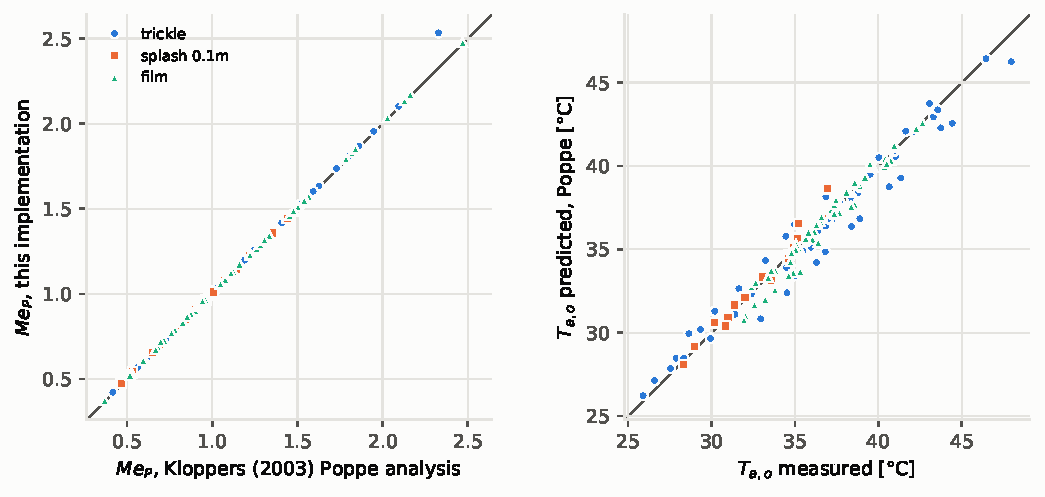
\includegraphics[width=\linewidth]{fig_kloppers_validation}
\caption{Poppe implementation against the fill tests of \citet{kloppers2003critical}. Left: Merkel number vs Kloppers'
Poppe analysis of the same tests. Right: predicted vs measured outlet-air temperature.}\label{fig:kloppers}
\end{figure}

%======================================================================
\section{Case studies}\label{sec:case}
%======================================================================
Three buildings were simulated in the same 14 climates (Table~\ref{tab:cases}). The primary case is the large data
center prototype developed by Lawrence Berkeley National Laboratory (LBNL) for the U.S. Department of Energy
(DOE)
\citep{sun2021prototype}, in its high-density version for ASHRAE Standard 90.1-2019 \citep{ashrae2019standard901}. It
was generated by the OpenStudio-Standards library \citep{openstudiostandards}; the model used here is that library's
output for climate zone 3A as archived by the Stor4Build project \citep{stor4build2024}, translated to EnergyPlus input
with the OpenStudio 3.7 Python bindings and converted to EnergyPlus 22.2 (the two input dictionaries differ in one
economizer field, which was dropped). The second case is the U.S. Department of Energy large office reference building
\citep{deru2011doe} as distributed with EnergyPlus. Both prototypes use a single-speed, fan-cycling tower sized by
EnergyPlus at fixed rating conditions, so the tower is the same at every site. They were changed in two respects only:
the tower evaporation mode was set to EnergyPlus' default saturated-exit formulation (the data center prototype uses the
loss factor), which does not affect the thermal solution, and the office was set to simulate the weather year (the
distributed file simulates design days only). The prototypes' envelopes, internal loads and controls were kept as
published, including the 3A envelope of the data center and the Chicago constructions of the office at every site,
because the purpose is to obtain realistic tower operating patterns rather than site-optimised buildings.

The third case is a 1\,MW data center with a three-cell variable-speed tower, developed in earlier work for this study
(supplementary file \url{https://github.com/TensorBuildLab/EnergyPlus-HeatRejection-Water/blob/main/models/DATACENTER_MODEL.md}). It represents the variable-speed towers common in new large
facilities and the other tower model of EnergyPlus, and it is the basis of the operating-point and sensitivity analyses
of Sections~\ref{sec:consistency} and~\ref{sec:sensitivity}. Design days and site data were replaced with each site's
ASHRAE values. Weather is TMYx 2011--2025 for 14 sites in ASHRAE climate zones 0A to 6A (zones from the weather files'
design conditions). EnergyPlus 22.2.0 was used.

\begin{table}[t]\centering\scriptsize
\caption{Case-study buildings. LBNL: Lawrence Berkeley National Laboratory; DOE: U.S. Department of Energy; COP:
chiller coefficient of performance. Tower operating hours, heat rejected and the share of heat rejected from October to
April are ranges over the 14 sites.}\label{tab:cases}
\begin{tabular}{p{0.17\linewidth}p{0.25\linewidth}p{0.25\linewidth}p{0.24\linewidth}}\toprule
 & Data center prototype & Office prototype & Data center, variable-speed tower \\\midrule
Source & LBNL/DOE large data center, high IT density, 90.1-2019 \citep{sun2021prototype,openstudiostandards} &
DOE large office reference building, new construction \citep{deru2011doe} & This study (supplementary model documentation) \\
Size and load & 557\,m$^2$, 3.0\,MW design IT, monthly IT schedule, 16,480\,MWh/yr IT & 46,320\,m$^2$, 12 floors and
basement, office schedules & 1,000\,m$^2$, 1.0\,MW design IT, 70--90\,\% utilisation \\
Chilled-water plant & 1 centrifugal chiller (COP 6.3), 6.7\,\textdegree C supply, integrated water-side economizer & 2
centrifugal chillers (COP 5.5), 6.7\,\textdegree C supply & 3 $\times$ 50\,\% variable-speed centrifugal, 10\,\textdegree C
supply \\
Tower & single speed, 2 cells, fan cycling; fan power at the 90.1-2019 minimum efficiency (40.2\,gpm/hp) & single speed, 1 cell, fan cycling & variable speed, 3 cells,
approach 3.9\,K at the site's 0.4\,\% wet-bulb \\
Condenser setpoint & $T_{wb}$ + 4.3\,K, 5.6--29.4\,\textdegree C & $T_{wb}$ + 0\,K (fan at full speed in 96--99\,\% of operating
hours) & $T_{wb}$ + 3.9\,K, 18--29.4\,\textdegree C \\
Tower operation & 8,760\,h; 22,800--23,700\,MWh; 59--62\,\% & 1,840--6,090\,h; 1,320--15,330\,MWh; 2--56\,\% & 8,760\,h;
9,250--9,590\,MWh; 57--58\,\% \\\bottomrule
\end{tabular}
\end{table}

%======================================================================
\section{Results}\label{sec:results}
%======================================================================
\subsection{The open-source plugin}\label{sec:tool}
The models are distributed as an EnergyPlus Python plugin with scripts that prepare any EnergyPlus model and analyse
its output (Fig.~\ref{fig:plugin}). The core is plain Python without third-party packages, so it runs in the Python
interpreter embedded in EnergyPlus. Using it takes three steps, which the repository's tutorial (\url{https://github.com/TensorBuildLab/EnergyPlus-HeatRejection-Water/blob/main/docs/TUTORIAL.md})
walks through with the data center prototype.
\begin{enumerate}
\item \emph{Install}: clone the repository from \url{https://github.com/TensorBuildLab/EnergyPlus-HeatRejection-Water}; EnergyPlus with Python plugin support (tested with version 22.2) is the only
requirement (the analysis scripts additionally use NumPy, pandas and Matplotlib).
\item \emph{Prepare}: \texttt{python tools/prepare\_model.py --idf building.idf --epw weather.epw --out run/} runs a
design-day sizing simulation to obtain the tower's design flows, reads every supported tower
(\texttt{CoolingTower:SingleSpeed}, \texttt{:VariableSpeed} and \texttt{:VariableSpeed:Merkel}), and writes a model with
the plugin objects (\texttt{PythonPlugin:SearchPaths}, \texttt{:Instance}, \texttt{:Variables} and
\texttt{:OutputVariable}) and output requests, plus a configuration file that names the makeup-water source, the treatment
limits and the chemistry mode (fixed cycles, constituent limits, or limits evaluated every timestep). Options select the
models, the loss factor and the climate-specific design days.
\item \emph{Run and analyse}: run EnergyPlus on the prepared model as usual. The results are ordinary output variables
per tower and timestep (Table~\ref{tab:outputs}); \texttt{tools/analyze.py} summarises a run and
\texttt{tools/scenarios.py} recomputes blowdown and makeup for other water sources and treatment programs without
re-simulation. \texttt{tools/run\_climates.py} runs one model in many climates in parallel.
\end{enumerate}
For the data center prototype the plugin with all eight models increases the run time of an annual simulation from 7\,s
to 109\,s (about 2\,ms per timestep on one core), most of it in the Poppe integrations; selecting fewer models reduces it
proportionally. The repository documents every equation with its source and code location (\url{https://github.com/TensorBuildLab/EnergyPlus-HeatRejection-Water/blob/main/docs/METHODS.md}),
contains 60 unit tests and reproduces every figure and table of this paper with one script. Appendix~\ref{app:code}
lists the plugin class and the input objects that the preparation step adds to a model.

\begin{figure}[t]\centering
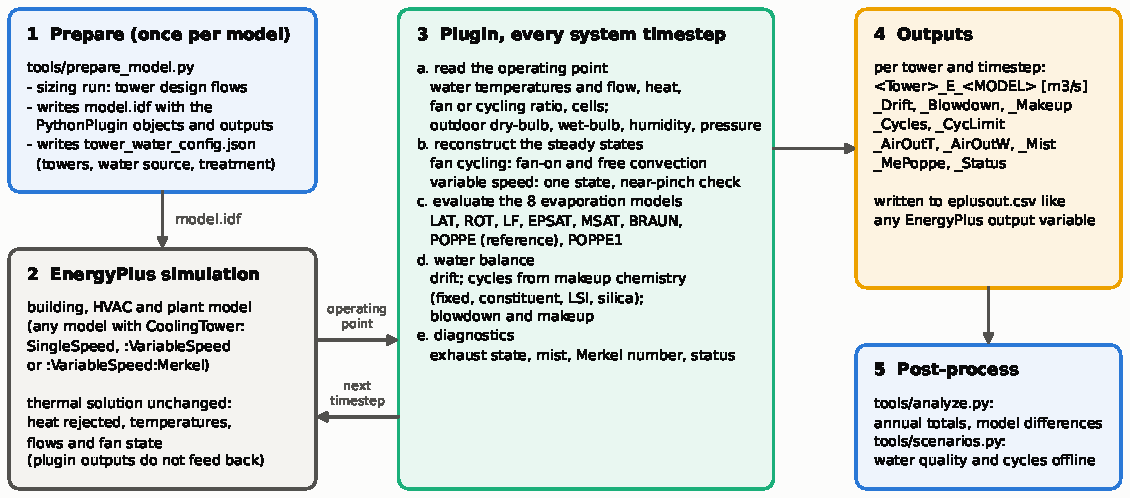
\includegraphics[width=\linewidth]{fig_plugin_workflow}
\caption{Workflow of the plugin. The model is prepared once; during the simulation the plugin reads the operating point
of each tower in every system timestep, reconstructs its steady states, evaluates all evaporation models and the water
balance, and writes the results as output variables without changing the thermal solution.}\label{fig:plugin}
\end{figure}

\begin{table}[t]\centering\small
\caption{Output variables written by the plugin for each tower (prefix = tower name), per system timestep.}\label{tab:outputs}
\begin{tabular}{ll}\toprule
Output & Content \\\midrule
\texttt{\_E\_LAT} \ldots\ \texttt{\_E\_POPPE1} & evaporation of each model [m$^3$/s] \\
\texttt{\_Drift}, \texttt{\_Blowdown}, \texttt{\_Makeup}, \texttt{\_MakeupVol} & water balance of the reference model
[m$^3$/s, m$^3$] \\
\texttt{\_Cycles}, \texttt{\_CycLimit} & cycles of concentration and the limiting constituent \\
\texttt{\_AirMass}, \texttt{\_AirOutT}, \texttt{\_AirOutW} & dry-air flow; exhaust temperature and humidity (Poppe) \\
\texttt{\_Fog}, \texttt{\_Mist} & supersaturated exhaust flag; liquid mist in the exhaust [m$^3$/s] \\
\texttt{\_MePoppe}, \texttt{\_MeMerkel}, \texttt{\_NTU} & Merkel numbers and transfer units implied by the operating point \\
\texttt{\_AirScale}, \texttt{\_Status} & near-pinch air-flow factor; solution status \\\bottomrule
\end{tabular}
\end{table}

\subsection{Where simplified models depart from Poppe}\label{sec:map}
To separate the physics from any building, a counterflow tower was sized with the Poppe model for a \SI{3.9}{K} approach
and \SI{5.6}{K} range at \SI{35}{\celsius}/\SI{25.6}{\celsius} and $L/G=1.2$ ($Me_P = 1.27$). With fill, $L/G$ and range
fixed, the cold-water temperature was solved with Poppe over a grid of dry-bulb (-5 to \SI{46}{\celsius}) and
relative humidity (5--100\,\%, wet-bulb below \SI{32}{\celsius}), and all models were evaluated at each point
(Fig.~\ref{fig:map}).

\begin{figure}[t]\centering
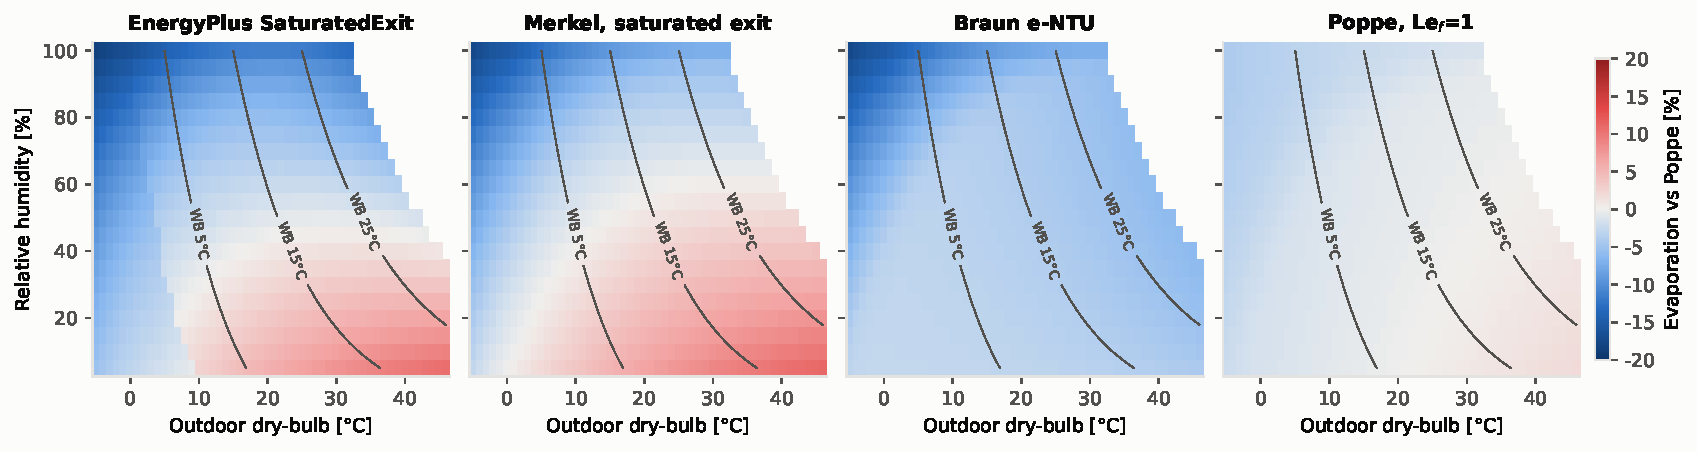
\includegraphics[width=\linewidth]{fig_method_map_physical}
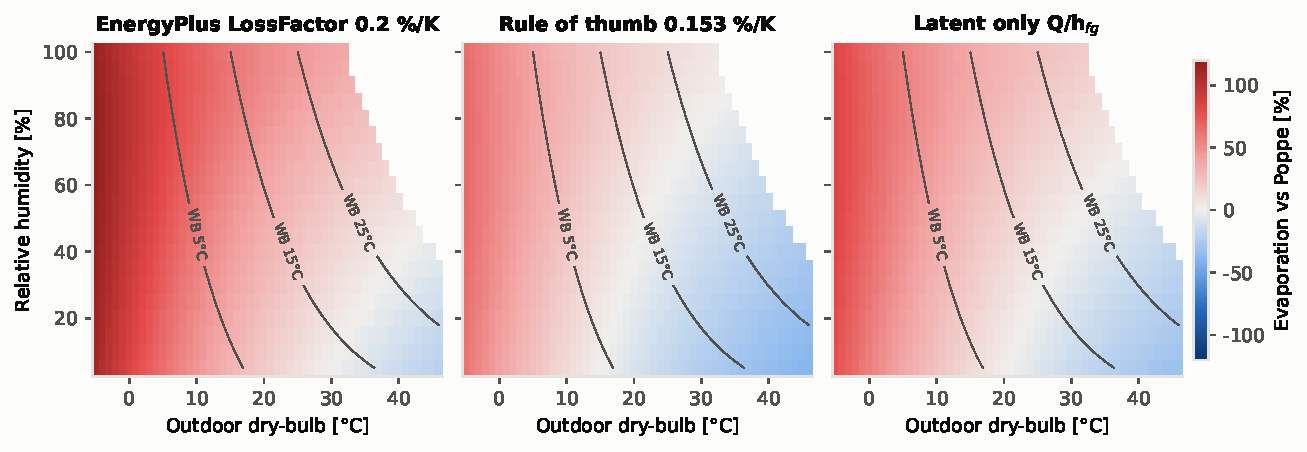
\includegraphics[width=0.8\linewidth]{fig_method_map_empirical}
\caption{Evaporation of each model relative to Poppe for a fixed tower at full load (top: $\pm$20\,\% scale; bottom:
$\pm$120\,\%). Lines: outdoor wet-bulb. Blank: wet-bulb above 32\,\textdegree C (not simulated). The step in the EnergyPlus
panel follows the 0\,\textdegree C wet-bulb line, where EnergyPlus switches its saturation-pressure formula from ice to
water.}\label{fig:map}
\end{figure}

Saturated-exit models differ from Poppe by -19 to +11\,\% (EnergyPlus' formulation -18.5 to +10.5\,\%, Merkel
-17.5 to +11.0\,\%). The sign follows the exhaust state predicted by Poppe. In hot, dry air the Poppe exhaust is
unsaturated, so a model that forces it to saturation adds water that does not evaporate, and saturated-exit models
overpredict. In cold, humid air the Poppe exhaust is supersaturated and carries liquid mist, which a saturated exhaust
cannot hold, and they underpredict. The Braun model gives 2.8--6.2\,\% less than Poppe where it can represent the
exhaust state, and down to -18\,\% where it is limited to saturated exit. The Lewis factor alone changes evaporation by
-4.2 to +1.8\,\%. Empirical models range from -39 to +117\,\%: they scale with the heat rejected or the range and
ignore the sensible share of the heat transfer. The latent-heat bound, for example, ranges from -32\,\% in hot, dry
air, where the air gives sensible heat to the water and more water evaporates than the heat rejected requires, to
+84\,\% in cold air, where much of the heat leaves as sensible heat.

The exhaust state also depends on the tower's operating point. At a given inlet state, more air per unit of water (a
lower $L/G$) leaves the exhaust further from saturation, which favours overprediction by saturated-exit models; less
air brings it closer to saturation or into supersaturation, which favours underprediction. At 40\,\textdegree C and
21\,\textdegree C wet-bulb with the map's approach and range, the EnergyPlus formulation gives 2\,\% more evaporation than
Poppe at $L/G=1.2$ but 5\,\% less at $L/G=1.64$. The annual results below follow directly from where each building's tower
operates in this space.

\subsection{Annual evaporation by building, tower control and climate}\label{sec:annual}
Table~\ref{tab:buildings} and Fig.~\ref{fig:buildings} compare the three buildings. The difference between the
EnergyPlus default and Poppe changes sign between them. For the variable-speed data center it is negative at every
site, -3.7\,\% (Phoenix) to -9.3\,\% (Montreal, Stockholm). For the office it ranges from -4.7\,\% (Singapore) to
+15.9\,\% (Las Vegas), and for the data center prototype from +2.4\,\% (Singapore) to +37.5\,\% (Riyadh). Within each
building the ranking of the climates is the same, from the largest overprediction in hot--dry climates (Riyadh, Las
Vegas, Phoenix, Madrid) to the smallest, or to underprediction, in hot--humid (Singapore, Mumbai, Houston) and cold
climates (Stockholm, Montreal).

The Merkel saturated-exit model (MSAT), which uses the physical air flow of each state, shows the physics alone. It is
-2.2 to -7.3\,\% for the variable-speed tower and -1.9 to +16.0\,\% for the two single-speed towers. The reason is the
air-to-water ratio. The variable-speed tower slows its fan at part load and runs at a median $L/G$ of 1.4--2.5, with
exhaust close to or beyond saturation; the single-speed towers run at their design $L/G$ of about 1.2--1.4 whenever the
fan is on, so in hot, dry air their exhaust leaves unsaturated (Section~\ref{sec:map}). The Braun model is 1.1--7.3\,\%
below Poppe in all three buildings, and the Lewis factor alone accounts for -2.1 to +4.5\,\%.

Evaporation per unit heat rejected (Poppe) is 1.04--2.13\,L/kWh$_{th}$ for the data center prototype, 1.42--2.76\,L/kWh$_{th}$
for the office and 1.05--1.65\,L/kWh$_{th}$ for the variable-speed data center, against about 1.48\,L/kWh$_{th}$ if all heat
left as latent heat. The office evaporates the most per unit heat in dry climates because its tower runs at full air flow
at part load and also cools the hot outdoor air, whose sensible heat is added to the evaporation. Consequently, the
empirical rules, which scale with heat or range, are wrong in a building-dependent way: the 0.2\,\%/K loss factor deviates
from Poppe by -19 to +65\,\% for the data center prototype and -38 to +22\,\% for the office, and the rule of thumb by
-38 to +26\,\% and -52 to -7\,\%.

\begin{figure}[t]\centering
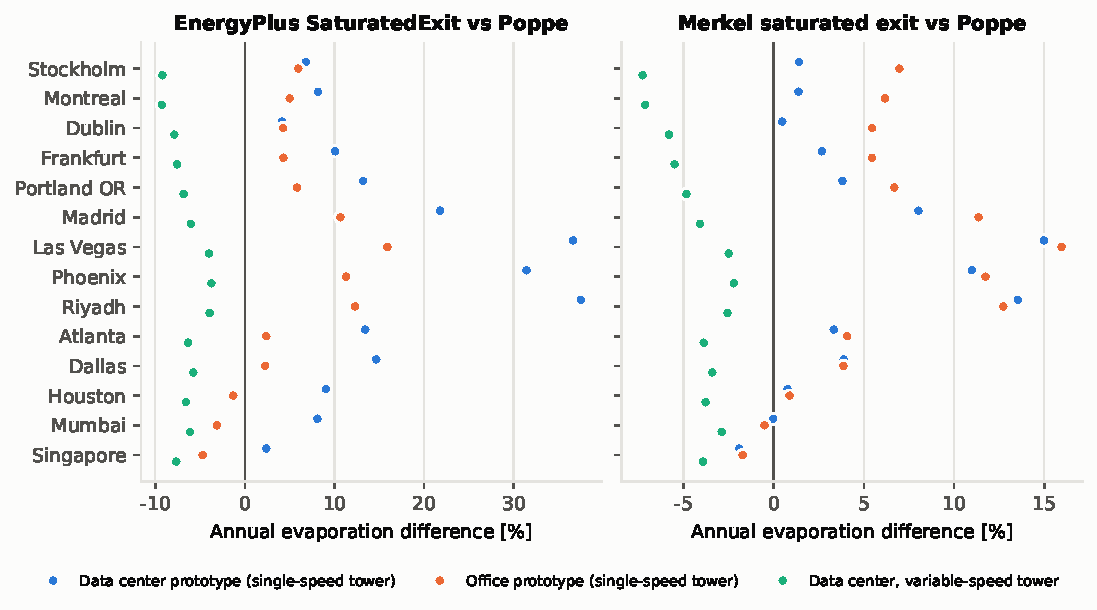
\includegraphics[width=\linewidth]{fig_buildings_deviation}
\caption{Annual evaporation of the EnergyPlus default (left) and of the Merkel saturated-exit model (right) relative to
Poppe, for the three buildings in 14 climates (sites sorted by mean wet-bulb of the data center sites). The left panel
contains the physics and EnergyPlus' averaging of fan cycling; the right panel the physics only.}\label{fig:buildings}
\end{figure}

\begin{table}[t]\centering\scriptsize
\caption{Annual evaporation per heat rejected with Poppe (L/kWh$_{th}$) and annual evaporation of the EnergyPlus default
(EPSAT) and of the Merkel saturated-exit model (MSAT) relative to Poppe [\%], by building and site (sorted by mean
wet-bulb; CZ: ASHRAE climate zone). VS: variable speed.}\label{tab:buildings}
\resizebox{\linewidth}{!}{\begin{tabular}{llrrrrrrrrr}
\toprule
 & & \multicolumn{3}{c}{Data center prototype} & \multicolumn{3}{c}{Office prototype} & \multicolumn{3}{c}{Data center, VS tower} \\
\cmidrule(lr){3-5}\cmidrule(lr){6-8}\cmidrule(lr){9-11}
Site & CZ & L/kWh$_{th}$ & EPSAT & MSAT & L/kWh$_{th}$ & EPSAT & MSAT & L/kWh$_{th}$ & EPSAT & MSAT \\
\midrule
Stockholm & 6A & 1.04 & +6.8 & +1.4 & 1.71 & +6.0 & +7.0 & 1.05 & -9.2 & -7.3 \\
Montreal & 6A & 1.08 & +8.2 & +1.4 & 1.80 & +5.0 & +6.2 & 1.09 & -9.3 & -7.1 \\
Dublin & 5A & 1.05 & +4.1 & +0.5 & 1.53 & +4.3 & +5.5 & 1.05 & -7.9 & -5.8 \\
Frankfurt & 4A & 1.17 & +10.1 & +2.7 & 1.72 & +4.3 & +5.5 & 1.11 & -7.6 & -5.5 \\
Portland OR & 4C & 1.23 & +13.2 & +3.8 & 1.88 & +5.8 & +6.7 & 1.13 & -6.8 & -4.8 \\
Madrid & 3B & 1.45 & +21.8 & +8.0 & 2.17 & +10.7 & +11.4 & 1.25 & -6.0 & -4.1 \\
Las Vegas & 2B & 2.03 & +36.6 & +15.0 & 2.76 & +15.9 & +16.0 & 1.50 & -4.0 & -2.5 \\
Phoenix & 1B & 1.95 & +31.4 & +11.0 & 2.58 & +11.3 & +11.7 & 1.54 & -3.8 & -2.2 \\
Riyadh & 1B & 2.13 & +37.5 & +13.5 & 2.49 & +12.3 & +12.7 & 1.65 & -3.9 & -2.6 \\
Atlanta & 3A & 1.32 & +13.4 & +3.3 & 1.66 & +2.4 & +4.1 & 1.22 & -6.3 & -3.9 \\
Dallas & 2A & 1.41 & +14.7 & +3.9 & 1.74 & +2.3 & +3.9 & 1.27 & -5.8 & -3.4 \\
Houston & 2A & 1.33 & +9.0 & +0.8 & 1.54 & -1.3 & +0.9 & 1.25 & -6.6 & -3.8 \\
Mumbai & 0A & 1.45 & +8.1 & -0.0 & 1.51 & -3.1 & -0.5 & 1.35 & -6.1 & -2.9 \\
Singapore & 0A & 1.36 & +2.4 & -1.9 & 1.42 & -4.7 & -1.7 & 1.30 & -7.7 & -3.9 \\
\bottomrule
\end{tabular}
}
\end{table}

\begin{figure}[t]\centering
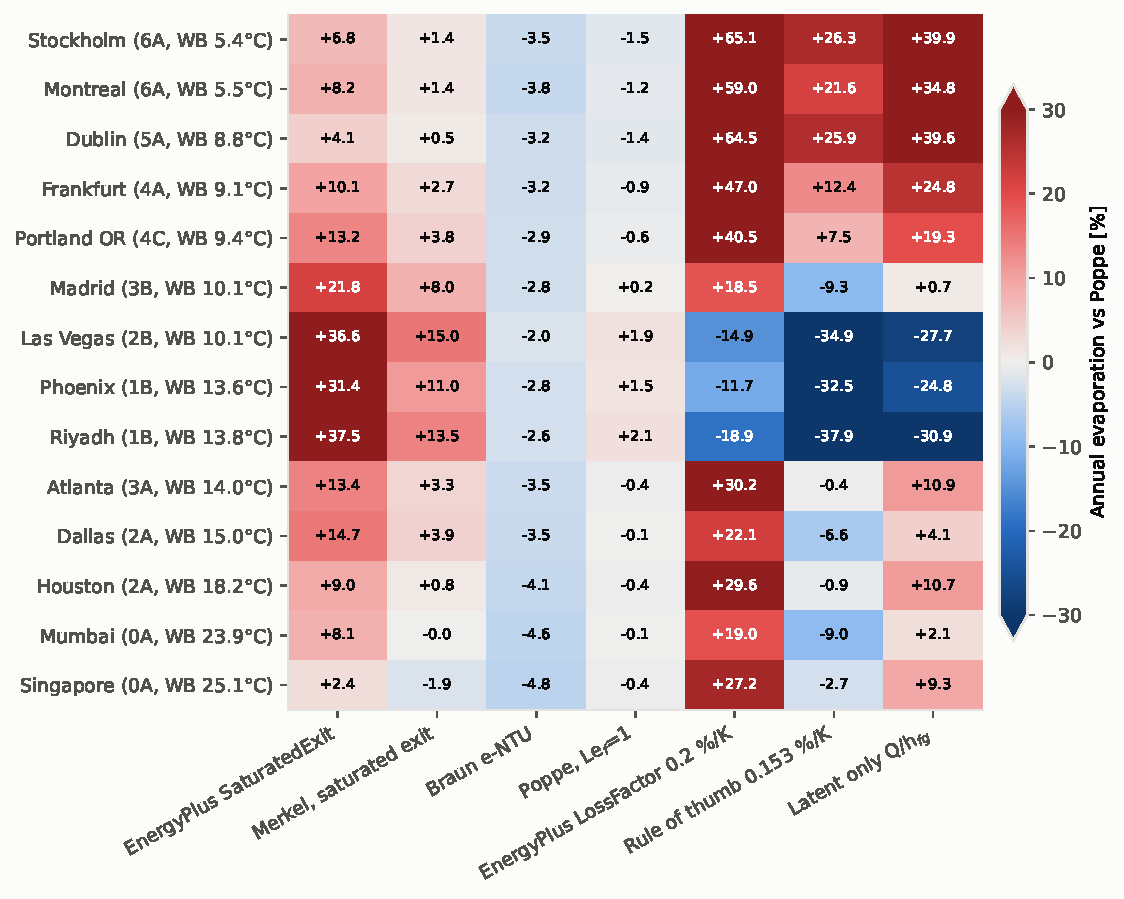
\includegraphics[width=\linewidth]{fig_proto_dc_method_deviation}
\caption{Annual evaporation of each model relative to Poppe (vapour and mist) for the data center prototype in 14
climates, sites sorted by mean wet-bulb. The colour scale is limited to $\pm$30\,\%; values are printed in each cell.}\label{fig:dcdev}
\end{figure}

\subsection{Averaging fan cycling over a timestep}\label{sec:cycling}
The tower of the data center prototype cycles its fan in 96--99.9\,\% of all hours, with the fan on for 68--79\,\% of the
time on average, because the integrated water-side economizer and the low condenser setpoint keep it working at part
load all year. The office tower cycles in only 1--4\,\% of its operating hours. For the data center prototype the
difference between the EnergyPlus default and Poppe splits into two parts. Applying the saturated-exit formula to each
of the two states and time-weighting the result, instead of applying the average heat to the full air flow, lowers
evaporation by 5.2--21.8\,\% of the Poppe value; this part is EnergyPlus' averaging convention. The remaining
saturated-exit physics contributes -5.1 to +14.2\,\%. For the office the averaging accounts for 0.6--2.1\,\% and the
physics for -6.1 to +13.7\,\%. Averaging matters because, at the full air flow, the saturated-exit formula assumes the whole
air stream is humidified to saturation even though the fan ran for only part of the timestep; in dry air this
humidification of air that did not pass through the tower is large. Poppe itself is insensitive to how the timestep is
represented: evaluating it once at the time-averaged air flow instead of at the two states changes annual evaporation by
-1.5 to -0.2\,\%.

\subsection{Vapour and liquid mist}\label{sec:mist}
In cold and mild climates Poppe predicts supersaturated exhaust in many hours. The liquid share of Poppe evaporation is
0.1--4.9\,\% for the variable-speed data center, largest at Stockholm, Montreal, Dublin and Frankfurt, but at most
1.5\,\% for the data center prototype and 0.1\,\% for the office, whose towers run with more air per unit water. Whether
this mist is consumed depends on how much of it the drift eliminators capture and return to the basin, so vapour-only
Poppe evaporation is a lower bound and total evaporation an upper bound. Against vapour-only Poppe the EnergyPlus default
differs by -7.4 to -3.5\,\% (variable-speed data center), +2.5 to +37.5\,\% (data center prototype) and -4.7 to
+15.9\,\% (office).

\subsection{Seasonal and timestep pattern}
Because the data center towers run all year, 57--62\,\% of their heat is rejected between October and April, and up to a
quarter below 0\,\textdegree C at Montreal; the office rejects 2--56\,\% of its heat in those months. At the timestep level
the largest underpredictions of the EnergyPlus default occur below 0\,\textdegree C, where Poppe exhaust is supersaturated,
and the largest overpredictions in hot, dry hours (Fig.~\ref{fig:dcts}). Empirical models do not follow this climate signal
(Fig.~\ref{fig:dcmonthly}): the loss factor gives nearly the same evaporation in every month.

\begin{figure}[t]\centering
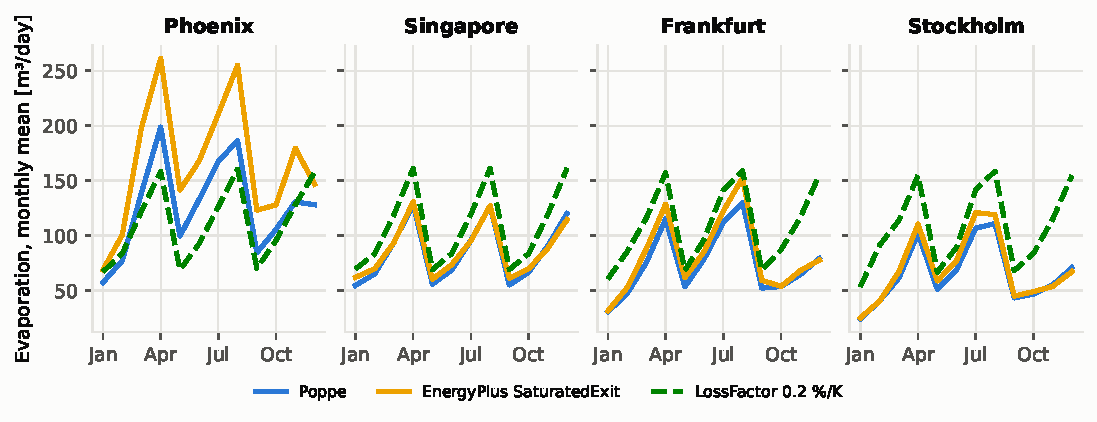
\includegraphics[width=\linewidth]{fig_proto_dc_monthly}
\caption{Monthly mean daily evaporation of the data center prototype: Poppe, EnergyPlus saturated exit and the
0.2\,\%/K loss factor.}\label{fig:dcmonthly}
\end{figure}

\begin{figure}[t]\centering
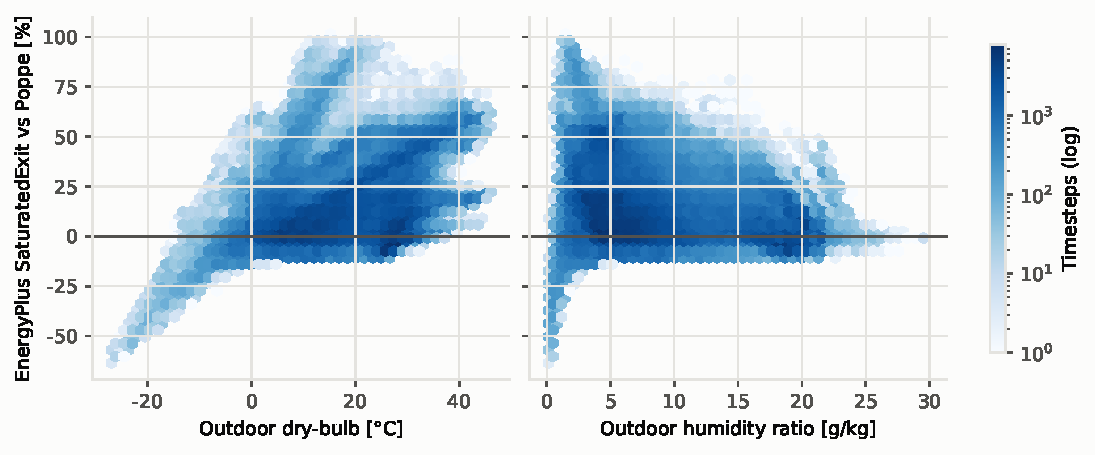
\includegraphics[width=\linewidth]{fig_proto_dc_timestep_deviation}
\caption{Timestep difference of the EnergyPlus default from Poppe (vapour and mist) against outdoor dry-bulb and
humidity ratio, data center prototype, all 14 sites.}\label{fig:dcts}
\end{figure}

\subsection{Dependence on the tower's thermal operating point}\label{sec:consistency}
Every model is evaluated at the air flow of EnergyPlus' tower model (Section~\ref{sec:samepoint}), so the results depend
on how EnergyPlus sizes and operates the tower. This was tested on the variable-speed data center, whose tower is
autosized for a 3.9\,K approach at each site's 0.4\,\% design wet-bulb with the condenser flow of three chillers (design
$L/G$ 1.6--1.8). Where the design wet-bulb is 21\,\textdegree C or lower (Dublin, Frankfurt, Madrid, Portland, Stockholm)
this design point is itself close to the pinch, with design Merkel numbers of 5.4--7.6 against 1.5--3.3 elsewhere
(Table~\ref{tab:fill}); at these sites the near-pinch correction of Section~\ref{sec:airflow} was needed in 66--100\,\% of
hours, with a mean air-flow factor of 1.02--1.03, and elsewhere in fewer than 0.3\,\% of hours.

The tower was then replaced by one with an ordinary fill: a design $L/G$ of 1.0, 1.2 or 1.4 (design $Me_P$ 1.0--2.7) at the
same design water flow and conditions, with $Me_P\propto(L/G)^{-0.6}$. For every loaded hour the air flow that this tower
needs to deliver EnergyPlus' leaving-water temperature was solved with Poppe, so the heat rejected is unchanged and only
the air flow differs; hours in which even the design air flow cannot reach that temperature are excluded (up to 14\,\% at
Houston and Mumbai). The ordinary tower runs with 11--45\,\% more air (median, design $L/G$ 1.2), and its Poppe evaporation
differs from the value at EnergyPlus' air flow by -0.1 to +6.4\,\%, most at hot--dry sites. At its operating point the
EnergyPlus formula differs from Poppe by -9.1 to -3.4\,\% at Stockholm, Montreal, Dublin, Frankfurt and Portland, by
-6.0 to +3.0\,\% at Madrid and the warm--humid sites, and by -2.0 to +10.9\,\% at Phoenix, Las Vegas and Riyadh, where the
sign depends on the design $L/G$. This is the same mechanism that separates the variable-speed and single-speed towers in
Section~\ref{sec:annual}: in cold and mild climates the underprediction is robust to the tower model, whereas in hot, dry
climates the sign depends on the tower's air-to-water ratio.

\begin{table}[t]\centering\scriptsize
\caption{Variable-speed data center: design point of the EnergyPlus tower and the ordinary-fill check (sites sorted by
mean wet-bulb). $T_{wb,d}$: design wet-bulb; $Me_{P,d}$: Poppe Merkel number at the design point; corr.: share of loaded
hours with the near-pinch air-flow correction; EP vs P: EnergyPlus saturated exit vs Poppe annual evaporation. Ordinary
fill: design $L/G$ = 1.2, and range over design $L/G$ = 1.0--1.4; P shift: Poppe evaporation with the ordinary fill vs
EnergyPlus' air flow; capped: hours excluded because the ordinary tower cannot reach EnergyPlus' leaving-water
temperature.}\label{tab:fill}
\resizebox{\linewidth}{!}{\begin{tabular}{lrrrrrrrrr}
\toprule
 & \multicolumn{4}{c}{EnergyPlus tower (base plant)} & \multicolumn{5}{c}{Ordinary fill, design $L/G$ = 1.0--1.4} \\
\cmidrule(lr){2-5}\cmidrule(lr){6-10}
Site & $T_{wb,d}$ & $Me_{P,d}$ & corr. & EP vs P & $Me_{P,d}$ & EP vs P & EP vs P & P shift & capped \\
 & [\textdegree C] & & [\% h] & [\%] & ($L/G$=1.2) & ($L/G$=1.2) [\%] & range [\%] & [\%] & [\% h] \\
\midrule
Stockholm & 20.0 & 7.6 & 100 & -9.3 & 2.05 & -8.9 & -9.1 to -8.5 & +0.3 & 0.0 \\
Montreal & 23.5 & 2.8 & 0 & -9.3 & 1.51 & -7.9 & -8.6 to -6.6 & +0.5 & 0.1 \\
Dublin & 20.0 & 7.2 & 99 & -7.9 & 2.07 & -7.7 & -7.8 to -7.3 & -0.0 & 0.0 \\
Frankfurt & 21.0 & 6.5 & 66 & -7.6 & 1.85 & -6.5 & -7.2 to -5.1 & +1.0 & 0.0 \\
Portland OR & 20.8 & 7.2 & 95 & -6.8 & 1.87 & -5.3 & -6.2 to -3.4 & +1.5 & 0.0 \\
Madrid & 20.0 & 5.4 & 66 & -6.0 & 2.01 & -4.0 & -5.4 to -1.3 & +2.4 & 0.0 \\
Las Vegas & 22.5 & 2.7 & 0 & -4.0 & 1.60 & +1.5 & -2.0 to +7.1 & +3.2 & 0.0 \\
Phoenix & 24.1 & 2.4 & 0 & -3.7 & 1.42 & +4.0 & -0.4 to +10.9 & +3.4 & 0.3 \\
Riyadh & 21.8 & 3.3 & 0 & -3.9 & 1.69 & +2.5 & -1.6 to +9.5 & +4.9 & 0.0 \\
Atlanta & 25.1 & 2.0 & 0 & -6.3 & 1.33 & -3.4 & -5.0 to -0.7 & +1.1 & 2.7 \\
Dallas & 25.8 & 2.0 & 0 & -5.8 & 1.26 & -1.6 & -3.9 to +2.0 & +1.5 & 8.5 \\
Houston & 26.8 & 1.8 & 0 & -6.7 & 1.17 & -3.2 & -5.1 to -0.3 & +1.1 & 13.1 \\
Mumbai & 28.4 & 1.5 & 0 & -6.3 & 1.05 & -0.9 & -3.5 to +3.0 & +1.4 & 13.8 \\
Singapore & 28.0 & 1.6 & 0 & -7.9 & 1.08 & -4.4 & -6.0 to -1.8 & +1.0 & 1.7 \\
\bottomrule
\end{tabular}
}
\end{table}

\subsection{Sensitivity}\label{sec:sensitivity}
For the variable-speed data center, sizing the tower for the two duty chillers instead of all three or lowering the condenser floor to
15\,\textdegree C changes the EnergyPlus--Poppe difference by up to 1.1 percentage points (Table~\ref{tab:sens}). A plant
built from the specifications of chillers and towers common in data centers (supplementary file \url{https://github.com/TensorBuildLab/EnergyPlus-HeatRejection-Water/blob/main/docs/EQUIPMENT_SPECS.md};
15.5\,\textdegree C chilled water, ASHRAE 90.1 centrifugal-chiller curves \citep{ashrae2019addendumbd}, a 15.5\,\textdegree C
condenser floor, a tower heat-transfer coefficient that scales with the air- and water-flow ratios to the powers 0.7 and
0.58, fitted to the fill data of \citet{kloppers2003critical}, a 0.25 minimum
fan speed and 50\,\% cell turndown) gives -8.4 to -2.5\,\%, 0.4--1.2 points smaller than the base plant. Plant variants of
the same tower type therefore preserve the sign and the ranking of the sites; changing the tower's air-to-water ratio,
through an ordinary fill or a single-speed tower, does not at hot--dry sites. Fill exponents of 0.5, 0.6 and 0.78 change
evaporation per unit heat by at most 0.17\,\% in a fixed-fill rating check at EnergyPlus' operating points. Over the
documented loss-factor range (0.15--0.27\,\%/K) the loss-factor estimate spans -22 to +122\,\% of Poppe across sites. Drift
(0.001\,\%) is below 0.2\,\% of makeup in all cases. Weather-year variability was not studied; a single typical year per site
was used.

\begin{table}[t]\centering\small
\caption{Variable-speed data center: EnergyPlus saturated exit vs Poppe annual evaporation [\%] for plant variants.
$^a$15.5\,\textdegree C chilled water and condenser floor, ASHRAE 90.1 chiller curves, fill-data heat-transfer curves, 0.25 minimum fan
speed, 50\,\% cell turndown. $^b$Same simulations as the base plant, tower replaced by an ordinary fill
(Section~\ref{sec:consistency}); hours the ordinary tower cannot meet are excluded. Variants with ``--'' were run only at
the four sites shown.}\label{tab:sens}
\begin{tabular}{lrrrrr}
\toprule
Plant variant & Phoenix & Singapore & Frankfurt & Stockholm & All sites ($n$) \\
\midrule
Base (N+1 tower, 18\,\textdegree C floor) & -3.7 & -7.9 & -7.6 & -9.3 & -9.3 to -3.7 (14) \\
Tower sized for duty (2 chillers) & -4.4 & -8.4 & -7.7 & -9.3 & -- \\
Condenser floor 15\,\textdegree C & -3.1 & -7.9 & -6.6 & -8.2 & -- \\
Both & -4.1 & -8.4 & -6.9 & -8.4 & -- \\
Equipment-informed plant$^a$ & -2.5 & -7.5 & -6.7 & -8.3 & -8.4 to -2.5 (14) \\
\bottomrule
\end{tabular}

\end{table}

\subsection{Makeup-water quality and water usage effectiveness}\label{sec:wue}
At four cycles, the WUE of the data center prototype is 1.93--4.08\,L/kWh$_{IT}$ with Poppe evaporation and
2.03--5.62\,L/kWh$_{IT}$ with the EnergyPlus default; for the variable-speed data center it is 1.72--2.74 and
1.57--2.63\,L/kWh$_{IT}$. With each site's own makeup water the allowable cycles, and hence blowdown, differ widely
(Table~\ref{tab:waterquality}, Fig.~\ref{fig:wue}). Soft supplies (Atlanta, Portland, Madrid, Singapore, Dublin, Stockholm)
reach 5.7--10 cycles; at Atlanta, Portland and Madrid every limit set reaches the model's 10-cycle cap (-17\,\%), partly
because sulfate, chloride or silica data are missing, so these results reflect the cap rather than the chemistry.
Supplies with moderate alkalinity (Dallas, Houston, Montreal, Mumbai) are limited by alkalinity unless acid is fed
(-14 to +3\,\% without capped cases). Frankfurt's hard water allows 2.3--4.7 cycles (-4 to +31\,\%) and Riyadh's
chloride 2.1--4.1 cycles (-1 to +44\,\%). Colorado River water at Phoenix and Las Vegas already carries 210--240\,mg/L
sulfate, so the 250\,mg/L sulfate limits of two galvanized-steel sets allow about one cycle, which the model raises to its
1.5-cycle floor (+125\,\%); such sites use stainless steel, acid feed or side-stream treatment, and the other three sets give
2.5--3.3 cycles (+7 to +25\,\%). Excluding cases at the cap or floor, site water changes makeup by -16 to +44\,\% relative
to four cycles. This is comparable to the evaporation-model effect, and the two multiply: the cycles of concentration are
an operating set-point, so site cycles, or the water quality and treatment program behind them, should be reported with
any simulated WUE. Soft, low-alkalinity waters are in practice limited by corrosion, which the model does not represent,
so their high-cycle results are optimistic. Data confidence is low for Atlanta, Madrid and Mumbai and low to medium for
Dallas.

\begin{table}[t]\centering\scriptsize
\caption{Data center prototype: site makeup water and cycles of concentration. Data: confidence of the water-quality data
(H high, M medium, L low); $^\dagger$sulfate, chloride or silica missing (treated as non-limiting). $N_{c,\mathrm{eff}}$:
effective annual cycles $E/(B+D_r)+1$, range over the five limit sets. $\Delta$WUE: Poppe makeup per IT energy relative to
four cycles, over all sets ($^c$lower end at the 10-cycle cap; $^f$upper end at the 1.5-cycle floor) and over the sets at
neither bound (``--'': none). ``min.'': raised to the 1.5-cycle minimum.}\label{tab:waterquality}
\resizebox{\linewidth}{!}{\begin{tabular}{lrrrrlrlrrr}
\toprule
Site & Ca & Alk. & SO$_4$ & Cl & Data & $N_{c,\mathrm{eff}}$ & Limit (lowest $N_c$) & WUE$_{N=4}$ & $\Delta$WUE, all sets & $\Delta$WUE, unclamped \\
 & \multicolumn{4}{c}{[mg/L; Ca, Alk.\ as CaCO$_3$]} & & & & [L/kWh] & [\%] & [\%] \\
\midrule
Atlanta & 8 & 12 & 4 & 3 & L & 10.0--10.0 & cap (10) & 2.47 & -17$^c$ to -17 & -- \\
Dallas & 105 & 110 & 33 & 20 & L--M & 3.6--7.6 & alkalinity & 2.66 & -14 to +3 & -14 to +3 \\
Dublin & 47 & 28 & 35 & 25 & M$^\dagger$ & 7.1--10.0 & sulfate & 1.95 & -17$^c$ to -13 & -13 to -13 \\
Frankfurt & 170 & 171 & 45 & 22 & M & 2.3--4.7 & alkalinity & 2.20 & -4 to +31 & -4 to +31 \\
Houston & 97 & 95 & 21 & 38 & M & 4.2--7.8 & alkalinity & 2.52 & -14 to -2 & -14 to -2 \\
Las Vegas & 187 & 112 & 209 & 99 & H & 1.5--3.2 & sulfate (min.) & 3.80 & +9 to +125$^f$ & +9 to +21 \\
Madrid & 40 & 40 & -- & -- & L$^\dagger$ & 10.0--10.0 & cap (10) & 2.74 & -17$^c$ to -17 & -- \\
Montreal & 77 & 93 & 22 & 26 & H & 4.3--10.0 & alkalinity & 2.00 & -17$^c$ to -2 & -11 to -2 \\
Mumbai & 35 & 97 & -- & 10 & L$^\dagger$ & 4.1--10.0 & alkalinity & 2.70 & -17$^c$ to -1 & -10 to -1 \\
Phoenix & 188 & 132 & 239 & 90 & M--H & 1.5--3.3 & sulfate (min.) & 3.72 & +7 to +125$^f$ & +7 to +25 \\
Portland OR & 5 & 29 & -- & -- & H$^\dagger$ & 10.0--10.0 & cap (10) & 2.30 & -17$^c$ to -17 & -- \\
Riyadh & 146 & 80 & 88 & 120 & M$^\dagger$ & 2.1--4.1 & chloride & 4.08 & -1 to +44 & -1 to +44 \\
Singapore & 39 & 35 & 7 & 30 & H & 8.3--10.0 & chloride & 2.52 & -17$^c$ to -15 & -15 to -15 \\
Stockholm & 65 & 45 & 44 & 16 & M--H$^\dagger$ & 5.7--10.0 & sulfate & 1.93 & -17$^c$ to -9 & -16 to -9 \\
\bottomrule
\end{tabular}
}
\end{table}

\begin{figure}[t]\centering
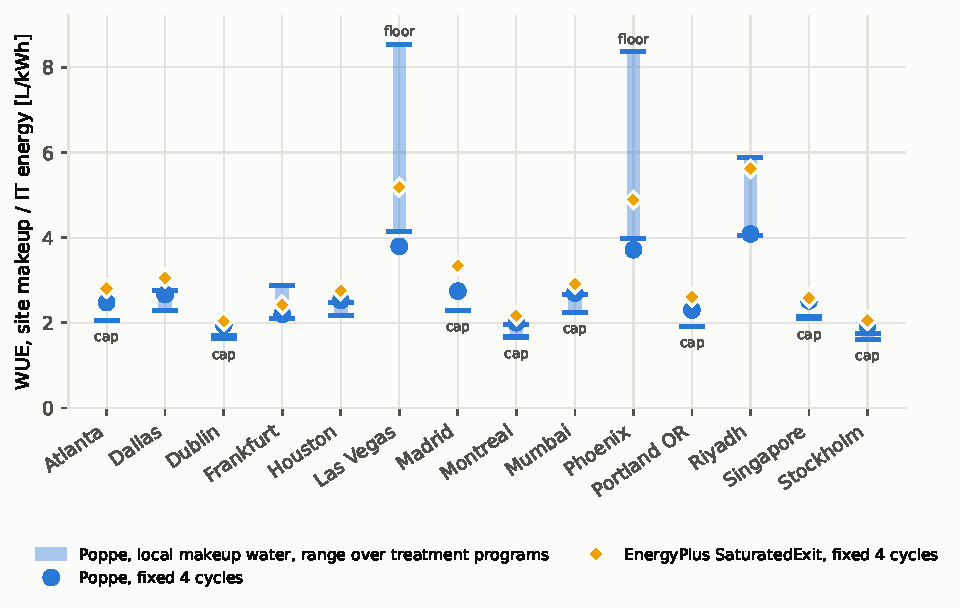
\includegraphics[width=\linewidth]{fig_proto_dc_water_quality}
\caption{WUE of the data center prototype by climate. Diamonds: EnergyPlus default (saturated exit, 4 cycles). Circles:
Poppe, 4 cycles. Bars: Poppe with each site's makeup water, range over five treatment limit sets; ``cap'' and ``floor''
mark range ends set by the model's 10-cycle cap or 1.5-cycle floor.}\label{fig:wue}
\end{figure}

%======================================================================
\section{Discussion}\label{sec:discussion}
%======================================================================
\subsection{What determines the error of simplified models}
The results reduce to one physical statement: the error of a simplified evaporation model is set by the state of the
air leaving the tower, and that state is set jointly by the weather and by how much air the tower moves per unit of water.
Climate alone does not determine the sign. The same hot, dry climate gives a 4\,\% underprediction for a variable-speed
tower that slows its fan and a 37\,\% overprediction for a single-speed tower that cycles at full air flow. For a building
model this means that the tower's part-load control and sizing are as important for the water estimate as the
evaporation model itself, and that a correction factor derived for one tower type or climate does not transfer to
another.

\subsection{Which model to use}
For annual totals in cold and mild climates, saturated-exit and e-NTU models are within about 10\,\% of Poppe and
consistently lower for variable-speed towers. In hot, dry climates, and for any fan-cycling tower, their error can exceed
30\,\% and its sign depends on the tower, so neither under- nor overestimation can be assumed; a model that resolves the
exhaust state, such as Poppe, and a timestep representation that resolves fan cycling are needed. At the timestep level the
differences are largest in freezing and in hot, dry weather, so hourly and peak water estimates need the full model.
Loss-factor and rule-of-thumb estimates scale with heat or range, deviate from Poppe by up to 65\,\% in either direction
depending on building and climate, and do not follow the seasonal signal; they should not be used for siting or
permitting. Because the mist share depends on drift eliminators, reporting vapour-only and total Poppe evaporation as a
range is recommended.

\subsection{Recommendations for data center water modeling}\label{sec:dcrec}
Data centers are the case in which the choice of model matters most, because their towers reject heat in every hour,
57--62\,\% of it between October and April, and economizers keep them at part load for most of the year. The results
lead to six recommendations. (i) For a fan-cycling tower, such as that of the LBNL/DOE prototype and of many plants
with water-side economizers, the EnergyPlus default should not be used for water estimates: it exceeded Poppe by 2 to
38\,\%, largely because of its averaging of fan cycling. Poppe, evaluated at the fan-on and free-convection states, is
needed; a saturated-exit model evaluated at the two states removes the averaging part of the error but not the physics
part. (ii) For a variable-speed tower in a cold or mild climate, the saturated-exit and e-NTU models give annual totals
within 10\,\% of Poppe and consistently below it, which is acceptable for early-stage estimates if this bias is stated.
(iii) Comparisons of WUE across sites, siting decisions and the choice between air-cooled, hybrid and evaporative heat
rejection should use Poppe, because the error of the simplified models changes by tens of percentage points between
climates and can change the ranking of sites. (iv) Hourly and peak water demand, which determine the size of the water
connection and the exposure to drought restrictions, should use Poppe, since the largest timestep differences occur in
freezing and in hot, dry hours. (v) Loss-factor and rule-of-thumb estimates should not be used for data centers: they
differed from Poppe by up to 65\,\% and do not follow the seasonal pattern of year-round operation. (vi) Simulated WUE
should be reported with the evaporation model, the tower control and the cycles of concentration or the makeup-water
quality and treatment program assumed, since site water alone changed makeup by -16 to +44\,\%.

\subsection{Beyond data centers and beyond EnergyPlus}
The physics is not specific to data centers. What distinguishes the building types is when and how the tower operates:
the data centers reject heat in every hour, including the freezing and humid hours in which saturated-exit models
underpredict, and the prototype's economizer keeps the tower at part load all year; the office tower runs mainly in warm
weather at full air flow. The same reasoning applies to hospitals, laboratories, district plants and industrial process
cooling, whose operating patterns lie between these cases. The method of evaluating all models at the simulated operating
point, with fan cycling resolved into its states, applies to any simulation program that reports the tower's operating
point, and the open-source implementation can be used directly with existing EnergyPlus models, including the prototype
buildings used in code development and in national building-stock studies.

%======================================================================
\section{Conclusions}\label{sec:conclusions}
%======================================================================
This study asked how much the choice of evaporation model changes the simulated water use of cooling towers, why, and
what this means for data centers. Eight models, from empirical rules to the Poppe model, were evaluated at the same
simulated operating point in every timestep, with the fan-on and free-convection states of fan-cycling towers resolved,
in an open-source EnergyPlus plugin. The implementation was verified against an independent solution and 126 measured
fill tests and applied to the LBNL/DOE large data center prototype, a data center with a variable-speed tower and the
DOE large office prototype in 14 climates.

The error of simplified models follows the state of the exhaust air. Saturated-exit models overpredict where hot, dry
air leaves the fill unsaturated and underpredict where cold air leaves it supersaturated; for a fixed tower at full load
they differ from Poppe by -19 to +11\,\%, and empirical rules by -39 to +117\,\%. Which regime dominates in a building
is decided by the tower's air-to-water ratio, that is, by its part-load control. In the 14 climates the EnergyPlus default
differs from Poppe by -9 to -4\,\% for the variable-speed tower, -5 to +16\,\% for the office prototype and +2 to +38\,\%
for the data center prototype. For fan-cycling towers, applying the timestep-average heat to the full air flow, as
EnergyPlus does, adds 5 to 22\,\% of the Poppe value to the evaporation of the data center prototype; resolving the two
states removes this, and Poppe itself is insensitive to how the timestep is represented. The Poppe implementation agrees
with the independent solution within 0.01\,\% and reproduces the measured outlet-air temperatures of the fill tests
better than saturated-exit analyses (0.84 against 1.10\,K root-mean-square error). With each site's own makeup water,
cycles of concentration set by sourced treatment limits change makeup by -16 to +44\,\% relative to four cycles, an
effect of the same order as the choice of evaporation model.

For practice, the results mean that data center water estimates used for design, siting, permitting and the choice
between air-cooled and evaporative heat rejection should use a model that resolves the exhaust-air state and the
part-load operation of the tower, such as Poppe, and should be reported together with the tower control and the cycles
of concentration assumed. Simplified saturated-exit models are adequate for annual totals of variable-speed towers in
cold and mild climates if their bias of up to -10\,\% is stated, whereas loss factors and rules of thumb should not be
used for data centers. Because the plugin works with existing EnergyPlus models, including the prototype buildings used
in code development and building-stock studies, these estimates can be obtained without changing the thermal model.

The study has limitations. All models are evaluated at the thermal operating point of EnergyPlus' tower models; with an
ordinary fill, Poppe evaporation for the same heat and leaving-water temperature differs from that value by up to
6.4\,\% at hot, dry sites. The fill tests measured outlet-air temperature rather than evaporation and covered only mild
inlet air with supersaturated exhaust, so the case-study comparisons are model to model, with Poppe as the most complete
model rather than ground truth. The prototypes were used as published, with one envelope for all sites and the office's
unreachable condenser setpoint, and one typical weather year was used per site. Makeup-water data are of low confidence
at four sites and incomplete at five; corrosion limits are not modelled; cycles are assumed to follow the water
temperature instantly; and the recirculating pH without acid feed is assumed.

Future work should therefore compare the models with metered makeup and blowdown of operating data center towers, in
particular in hot, dry and in freezing climates; couple a tower model with a Poppe thermal solution and a characterised
fill to the building simulation; and extend the analysis to multi-year and future weather, to corrosion-limited water
treatment and to hybrid and air-cooled heat rejection, so that the long-term water and energy consequences of the cooling
system chosen for a new data center can be compared on a consistent basis.

%======================================================================
\section*{CRediT authorship contribution statement}
\textbf{Liang Zhang:} Conceptualization, Methodology, Software, Validation, Formal analysis, Investigation, Data
curation, Visualization, Writing -- original draft, Writing -- review \& editing, Funding acquisition.

\section*{Declaration of competing interest}
The author declares no known competing financial interests or personal relationships that could have
appeared to influence the work reported in this paper.

\section*{Declaration of generative AI and AI-assisted technologies in the manuscript preparation process}
During the preparation of this work the author used Claude (Anthropic) in order to assist with software development,
data analysis scripts, literature and reference checking, and drafting and language editing of the manuscript. After
using this tool, the author reviewed and edited the content as needed and takes full responsibility for the content of
the published article.

\section*{Acknowledgements}
This material is based upon work supported by the U.S. National Science Foundation under Award No. 2623038. Any
opinions, findings, and conclusions or recommendations expressed in this material are those of the author and do not
necessarily reflect the views of the National Science Foundation.

\section*{Data availability}
The plugin, a tutorial, the building models, weather metadata, makeup-water data, run archive and the scripts that
reproduce every figure and table are openly available at
\url{https://github.com/TensorBuildLab/EnergyPlus-HeatRejection-Water} under the MIT licence;
\texttt{reproduce.sh} regenerates all results with EnergyPlus 22.2.0. Implementation issues in EnergyPlus' tower water
accounting found during this work are documented, with reproductions, in the repository
(\url{https://github.com/TensorBuildLab/EnergyPlus-HeatRejection-Water/tree/main/bugreports}).

\appendix
\section{Plugin code}\label{app:code}
The plugin is a Python class derived from EnergyPlus' \texttt{EnergyPlusPlugin}. EnergyPlus calls its method
\texttt{on\_end\_of\_system\_timestep\_before\_hvac\_reporting} at the end of every system timestep. The method reads the
tower and weather output variables through the EnergyPlus application programming interface, evaluates the models and
writes the results to plugin variables, which EnergyPlus reports like its own output variables. The listing below is
abridged from \texttt{src/tower\_water/eplus\_plugin.py} in the repository (error handling, the handle look-up and the
model evaluation in \texttt{compute\_tower} are omitted).
\begin{verbatim}
from pyenergyplus.plugin import EnergyPlusPlugin

class TowerWaterPlugin(EnergyPlusPlugin):
    CONFIG_PATH = None              # set by tools/prepare_model.py

    def __init__(self):
        super().__init__()
        with open(self.CONFIG_PATH) as fh:
            self.cfg = json.load(fh)    # towers, design flows, water, treatment
        self.towers = [setup_tower(t, self.cfg) for t in self.cfg["towers"]]
        self.ready = False

    def on_end_of_system_timestep_before_hvac_reporting(self, state):
        x = self.api.exchange
        if not self.ready:              # look up variable handles once
            if not x.api_data_fully_ready(state):
                return 0
            self._get_handles(state)
            self.ready = True
        site = {k: x.get_variable_value(state, h)
                for k, h in self.site.items()}   # dry-bulb, wet-bulb, w, p
        dt_s = x.system_time_step(state) * 3600.0
        for t in self.towers:
            v = {k: x.get_variable_value(state, h)   # temperatures, flow,
                 for k, h in t["_in"].items()}       # heat, fan state
            out = compute_tower(t, v, site, self.cfg, self.methods)
            out["MakeupVol"] = out["Makeup"] * dt_s
            for name, h in t["_out"].items():        # E_POPPE, Makeup, ...
                x.set_global_value(state, h, out[name])
        return 0
\end{verbatim}
The preparation step adds input objects of the following form to the EnergyPlus model (shortened; \texttt{CT1} stands
for the tower name, and one \texttt{PythonPlugin:OutputVariable} is written for every output of Table~\ref{tab:outputs}):
\begin{verbatim}
PythonPlugin:SearchPaths, TowerWater Paths, Yes, Yes, No,
    <repository>/src, <run directory>;
PythonPlugin:Instance, TowerWater, No,
    tower_water_model_plugin, ModelTowerWater;
PythonPlugin:Variables, TowerWater Vars 1,
    CT1_E_LAT, CT1_E_ROT, CT1_E_LF, CT1_E_EPSAT, CT1_E_MSAT,
    CT1_E_BRAUN, CT1_E_POPPE, CT1_E_POPPE1, CT1_Drift, CT1_Blowdown;
PythonPlugin:OutputVariable, CT1_E_POPPE, CT1_E_POPPE,
    Averaged, SystemTimestep, m3/s;
Output:Variable, CT1_E_POPPE, PythonPlugin:OutputVariable, Timestep;
\end{verbatim}

\bibliographystyle{elsarticle-num}
\bibliography{references}
\end{document}
